\documentclass[12pt]{report}

\usepackage[italian]{babel}
\usepackage[T1]{fontenc}
\usepackage[utf8]{inputenc}
\usepackage{algorithm}
\usepackage[noend]{algpseudocode}
\usepackage[pdftex]{graphics}
\usepackage{graphicx}
\graphicspath{/home/paologio/Documenti/Università/Tesi/Malchiodi/ACSDI/Elaborato}
\usepackage{chngcntr}
\counterwithout{footnote}{chapter}
\usepackage{booktabs}

\begin{document}

\tableofcontents

\chapter{Le reti neurali artificiali}

\linespread{1.4}\selectfont
\section{Definizione e origini storiche}
L’intuizione di replicare l’attività neurale che avviene nel cervello umano quando apprende, risale agli inizi degli anni ‘40, quando venne teorizzato un primo modello di neurone da McCulloch e Pitts (1943) [artificial intelligence a modern approach, pag. 728]. Il parallelo è molto stretto: così come il compito di un neurone è quello di ricevere, elaborare e ritrasmettere impulsi elettrici all’interno del sistema nervoso cerebrale, quello di un neurone artificiale è ricevere un certo dato in input ed attivarsi o meno in base alla propria "importanza" (peso assegnato ai propri collegamenti in entrata) e alla sua funzione di attivazione (di cui si parlerà in seguito).

\begin{figure}
\begin{center}
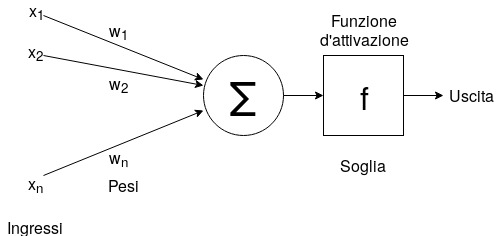
\includegraphics[scale=0.75]{neurone_artificiale.png}
\caption{Immagine di un neurone artificiale}
\end{center}
\end{figure}

\section{Applicazioni}
Le reti neurali vengono impiegate nell’attività di previsione (regressione) o classificazione.
Nel primo caso rientrano, ad esempio, le previsioni di vendita: riuscire a prevedere il prezzo di un immobile in base a fattori che lo descrivono (i metri quadrati, il numero di stanze, la posizione centrale o meno in un centro abitato, ecc…) o prevedere l’andamento di un titolo azionario in borsa.
Altro problema è quello invece della classificazione: si richiede, in questo caso, che la rete, dato un oggetto, ne restituisca la classe di appartenenza; tipico esempio è quello della classificazione di numeri scritti a mano o, date una serie di immagini, riconoscere quelle in cui è presente un particolare soggetto.
In questo elaborato si andrà ad affrontare il problema legato alla regressione.

\section{Architettura di una rete neurale}
Una rete, per essere definita tale, deve essere composta da almeno 3 strati:
\begin{enumerate}
\item{input}
\item{hidden}
\item{output}
\end{enumerate}

\begin{figure}
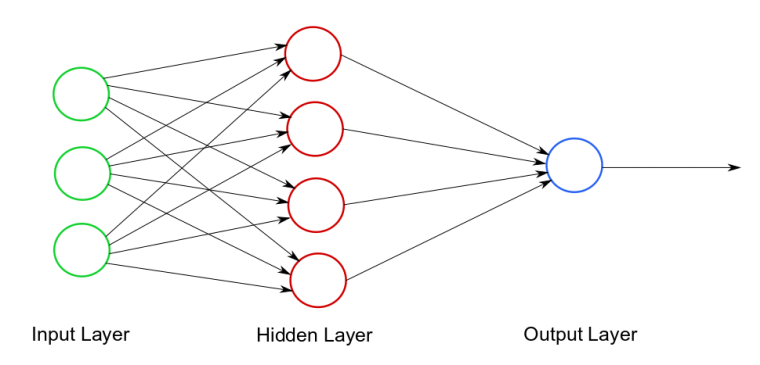
\includegraphics[scale=0.5]{nn_arch.png}
\caption{Architettura rete neurale}
\end{figure}

Il ruolo dello strato di input è quello di ricevere le features da elaborare, lo strato nascosto si occuperà di introdurre non linearità nel modello e renderlo capace di imparare pattern complessi e lo strato di output dovrà predire il risultato in base all’input ricevuto.

Inoltre, in base a come i neuroni dei vari strati sono collegati tra loro si possono distinguere due configurazioni di rete come quella densamente connessa (fully connected) o convoluzionale (convolutional).

In questo elaborato ci si concentrerà sulla tipologia densamente connessa, ossia, ogni neurone di uno strato sarà collegato ad ogni neurone del successivo.

\subsection{Componenti}
Come detto sopra, la rete è composta da strati; gli strati, a loro volta, sono un insieme di neuroni, ognuno dei quali ha associato un peso ($w$) per ogni collegamento in entrata e un bias ($b$). Questi sono stati impostati randomicamente, in un intervallo tra 0 e 1. Questi due sono gli unici parametri che, una volta inizializzati, vengono modificati automaticamente dalla rete durante il training. I restanti parametri, invece, rimangono tali durante tutte le fasi di addestramento del modello; inoltre l'unico modo per individuare tali parametri è empiricamente: questi prendono il nome di \textbf{\textit{iperparametri}}.

\section{Algoritmo feedforward}
Le connessioni tra i neuroni di uno strato e quelli del successivo sono monodirezionali, configurazione che porta ad avere un grafo diretto e aciclico. Quindi il flusso di dati che scorre nella rete viaggia dallo strato di input a quello di output senza che ci siano loop, il che implica anche che non ci siano interazioni tra neuroni dello stesso strato.

\subsection{Il calcolo tra strati}
Nell'implementazione pratica viene usata una matrice dei pesi per rappresentare le connessioni tra strati. 
Siano 
\begin{itemize}
\item{$W_{ih}$} la matrice dei pesi che rappresenta le connessioni tra strato input e hidden
\item{$W_{ho}$} la matrice dei pesi che rappresenta le connessioni tra strato hidden e output
\item{$b_h$} il vettore dei bias dello strato hidden
\item{$b_o$} il vettore dei bias dello strato di output
\item{$x$} il vettore di input
\item{$f$} la funzione d'attivazione scelta per lo strato
\end{itemize}
Per eseguire l'algoritmo di feed-forward occorre calcolare
$$\alpha = f\left(x \cdot W_{ih} + b_h\right)$$
Una volta ottenuto $\alpha$ si procede analogamente con lo strato successivo
$$prediction = f\left(\alpha \cdot W_{ho} + b_o\right)$$
Dato che la rete usata per fare regressione ha un solo neurone nello strato di output, $prediction$ sarà un unico valore e sarà la previsione della rete in base all'input ricevuto.

\section{Addestramento di una rete neurale}
Per continuare il parallelo con una rete neurale umana, così come per l'attività di apprendimento occorre studiare, anche una rete neurale artificiale ha bisogno di "studiare": questa fase viene detta fase di addestramento (training).
Una volta selezionato il dataset contenenti i caratteri che la rete dovrà apprendere, si procede a dividere tale insieme in due sottoinsiemi:

\begin{itemize}
\item{training set}
\item{testing set}
\end{itemize}

Il primo verrà usato per l'attività di apprendimento (solitamente si usa circa l'80\% dell'intero dataset estraendo casualmente esempi), il secondo per testare la bontà della rete su esempi che non ha ancora visto.

\subsection{Fase di training}
In questa fase, per ogni esempio nel training set, vengono date in input le features allo strato di input della rete. Tramite l'algoritmo di feed-forward (verrà spiegato successivamente) la rete propaga il risultato fino al neurone di output. È in questo momento che la rete impara elaborando le features e confrontando la previsione con l’effettivo target: in base alla differenza tra previsione e target effettivo, la rete stessa correggerà i pesi degli strati hidden usando un algoritmo di back-propagation (verrà spiegato successivamente).
Questa operazione viene eseguita un numero n di volte, numero che prende il nome di epoca. Un epoca può essere per ogni esempio di training (un’epoca termina quando è stato applicato feedforward e backprop per ogni esempio) oppure per un batch size (vengono considerati più esempi nella stessa iterazione, ad esempio con 1000 esempi e un batch size di 500 un epoca termina dopo 2 iterazioni).
Una volta che la rete ha iterato per un numero pari al numero di epoche scelto termina la fase di training.

\subsection{Fase di testing}
Terminata la fase di training occorre verificare il comportamente della rete su dati nuovi rispetto a quelli usati in training. Questo permette di capire la reale capacità di previsione della rete e se, durante la fase precedente, si sono verificati problemi di 
\begin{itemize}
\item{\textbf{\textit{overfitting}}}: si verifica quando il modello si adatta così tanto agli esempi del training set da perdere la capacità di generalizzare su nuovi esempi. Sintomo dell'overfitting è un'alta accuratezza durante la fase di training ed una scarsa accuratezza in fase di testing; la rete ha imparato "a memoria" i casi di training in modo tale da non riconoscerne di nuovi.
\item{\textbf{\textit{underfitting}}}: è l'opposto del caso precedente. Si verifica quando il modello non riesce ad imparare il pattern domimante nei dati di train, risultando in previsioni poco accurate.
\end{itemize}

\section{Algoritmo di back-propagation}
Una volta che l’informazione ha raggiunto lo strato di output ho la previsione; tuttavia questa conterrà dell’errore. Per ridurlo si usa un apposito algoritmo di propagazione all’indietro che regola i pesi associati ai collegamenti tra singoli neuroni, partendo dallo strato più esterno a quello più interno.

Si parte calcolando la loss function dell’output, che può essere l’errore medio assoluto (scelta fatta per gli esperimenti dell'elaborato) o l’errore quadratico medio, e se ne calcola la derivata parziale rispetto ai pesi dei collegamenti dei neuroni di output. A questo risultato si moltiplica il learning rate e si sottrae al peso $$W^n_x = W_x - \eta \left(\frac{\delta Error}{\delta W_x}\right)$$ dove $W^n_x$ è il valore del nuovo peso, $W_x$ il vecchio peso, $\eta$ il learning rate e tra parentesi $\frac{\delta Error}{\delta W_x}$ la derivata parziale dell'errore rispetto ai pesi. 

Una volta fatto questo calcolo con la matrice dei pesi strato hidden/output, si fa la stessa cosa per quella input/hidden.

\subsection{Iperparametri}\label{iperparametri}
In questa categoria rientrano:
\begin{itemize}
\item{learning rate}: indica il grado con cui la rete modifica i propri pesi durante la fase di back-propagation. Negli esperimenti di cui si parlerà in questo elaborato sono stati usati diversi learning rate ed ogni volta verranno specificati
\item{numero di epoche}: indica il numero di volte che la rete compie un passo di feed-forward e back-propagation (indipendentemente dal batch size)
\item{batch size}: indica la quantità di esempi presi in considerazione per la fase di feed-forward
\item{numero di neuroni per strato}: indica il numero di neuroni per singolo strato
\item{funzione d'attivazione}: funzione che attiva o meno il singolo neurone in base alla formula $$\Sigma\left(weight * input\right) + bias$$
\end{itemize}

\section{Model selection}
Come detto al paragrafo \ref{iperparametri}, per trovare il valore degli iperparametri bisogna basarsi su prove empiriche. In particolare in questo elaborato si sono fissati numero di epoche, batch size, numero di strati nascosti, learning rate e funzione d'attivazione mentre per il numero di neuroni per lo strato nascosto si è deciso di fare della model selection, in particolare usando una tecnica della \textbf{\textit{model selection}}: la \textbf{\textit{nested cross validation}}.

\subsection{Cross validation annidata}
Una volta aver diviso il training set dal testing set, viene utilizzato esclusivamente  il primo per la cross-validation. In particolare questo viene partizionato in k sottoinsiemi (fold) di cui uno di questi prenderà il nome di validation set e gli altri di training set. La rete verrà quindi allenata sui training set e poi testata sul validation set; a questo punto si sceglierà una diversa permutazione di fold in cui il validation set sarà shiftato di una posizione, fino a che tutte saranno esaurite. 
Es.: se il training set venisse suddviso in 3 fold le permutazioni prese in considerazione saranno:
\begin{enumerate}
\item{TRAINING | TRAINING | VALIDATION}
\item{TRAINING | VALIDATION | TRAINING}
\item{VALIDATION | TRAINING | TRAINING}
\end{enumerate}

Alla fine di ogni fold viene salvato l’errore della rete che verrà usato al termine delle permutazioni: verrà calcolato l’errore medio e, per ogni carattere su cui si fa model selection, si sceglierà l’architettura con l’errore minore. A questo punto si può riaddestrare e testare la rete che ha ottenuto il risultato migliore, oppure salvarsi di volta in volta, insieme al miglior risultato anche l’architettura che l’ha ottenuto; in questo elaborato si è scelta la prima soluzione.

Quella spiegata è la procedura di cross-validation: tuttavia quella usata in questo elaborato è una tipologia innestata. Quello che cambia è che, le operazioni viste sopra, che ora prenderanno il nome di fold interno, vengono ripetute j volte, dove j è il numero di fold esterno. Di seguito è presentato lo pseudo codice per una procedura di nested-cross-validation.

\makeatletter
\def\BState{\State\hskip-\ALG@thistlm}
\makeatother

\begin{algorithm}
\caption{Nested Cross Validation}
\begin{algorithmic}[1]
\Procedure{NestedCrossValidation}{}
\BState \emph{input}:
\State $H \gets \textit{insieme di iperparametri presi in considerazione}$
\State $S \gets \textit{training set}$
\State $K \gets \textit{numero di fold esterni}$
\State $J \gets \textit{numero di fold interni}$
\BState \emph{procedure}:
\State $S_{perm} \gets \textit{K permutazioni di S}$
\For {$k \in \{1,\dots,K\}$}
\State $s_{k} \gets \textit{k-esima permutazione di S}$
\State $L_M \gets \infty$

\For {$h \in H$}
\For {$j \in \{1, \dots, J\}$}
\State $s_{kj} \gets \textit{singola permutazione kj}$
\State $\textit{alleno la rete sul training set di} s_{kj}$
\State $\textit{valuto la rete sul validation set di} s_{kj}$
\State $L_j \gets \textit{valore di loss per il j-esimo fold}$
\EndFor
\State $L_{mean} \gets \textit{media delle loss} L_j$
\State $L_M \gets L < L_{mean} ? L : L_{mean}$
\EndFor
\State $Best[k] \gets \textit{risultato migliore per il k-esimo fold}$
\EndFor
\State $\textit{Per ogni iperparametro ho il carattere migliore dei k fold}$
\EndProcedure
\end{algorithmic}
\end{algorithm}

\chapter{Algoritmi di compressione per reti neurali}

\section{Compressione di una rete}

Uno degli svantaggi più evidenti delle reti neurali è lo spazio che questa occupa in memoria e i tempi elevati per l’addestramento. Aspetto che ha assunto un ruolo sempre più importante con il diffondersi di macchine con ridotte capacità di computazione e di memoria e in generale dell’IoT. 
Per ridurre questo impatto negativo si stanno studiando diversi metodi per comprimere le strutture dati utilizzate in modo da ridurre le dimensioni in memoria lasciando il più possibile invariata l’accuratezza della rete. Tale obiettivo è anche quello che si prefigge questo elaborato, ossia verificare l’efficacia di tecniche di compressione quali pruning e weight sharing su una rete neurale per il problema della regressione. 

\section{Pruning}

L’idea di fondo del pruning è semplice; ogni collegamento tra neuroni ha associato un peso che ne determina l’importanza (avrà letteralmente un peso maggiore nell’influenzare il risultato finale della rete), da qui l’intuizione per cui, ignorando i collegamenti con peso tendente allo zero, non altero significativamente il risultato della rete che otterrei considerandoli. 
Si sceglie quindi di eliminare questi neuroni alleggerendo così la matrice dei pesi da memorizzare; tuttavia questa operazione non è del tutto gratuita. A spese di una dimensione minore, ci si ritrova con nuove strutture dati con cui è più lenta l'operazione di moltiplicazione tra matrici. Come nuova struttura dati si può utilizzare una matrice
\begin{itemize}
\item{\textbf{\textit{Compressed Sparse Row}}}: vengono usati 3 vettori contenenti rispettivamente i valori non zero letti per riga, un puntatore alle righe e gli indici di colonna
\item{\textbf{\textit{Compressed Sparse Column}}}: simile alla precedente con la differenza che, nel primo vettore, i valori vengono letti per colonna, vengono memorizzati gli indici di riga per ogni valore, e i relativi puntatori alle colonne.
\end{itemize}


In questo elaborato la soglia per scartare i pesi è stata calcolata come n-esimo percentile rispetto la matrice dei pesi, dove n va da 10 a 90 con scalini di 10 (quindi con il 10\% verranno scartate il 10\% circa delle connessioni tra due strati comunicanti e così via).

\section{Weight Sharing}

L’obiettivo del weight sharing è quello di ridurre lo spazio necessario alla memorizzazione delle matrici dei pesi della rete; per fare ciò si raggruppano pesi simili in un singolo valore (peso che riesca a rappresentare adeguatamente i pesi che vi rientrano). Questo valore prende il nome di centroide e verrà usato in sostituzione ai pesi raggruppati per le operazioni matriciali. 

Per gli esperimenti trattati nell'elaborato, dopo aver fissato il numero di clusters per strato e dopo averne trovato i centroidi, le matrici dei pesi sono state sostituite con le matrici di indici che puntano al relativo centroide. \\
Per stabilire i centroidi si possono usare algoritmi di clustering; in particolare quello usato in questo elaborato è K-Means. 

\subsection{Algoritmo K-Means}
K-Means
L’algoritmo usato è quello della libreria sklearn, MiniBatchKMeans, che da documentazione segue l’euristica di Lloyd.

\begin{enumerate}
\item{Vengono scelti k centroidi casualmente, dove k è il numero di clusters che si vogliono creare}
\item{Ogni osservazione viene assegnata ad uno dei centroidi in base alla distanza euclidea dello stesso}
\item{I centroidi vengono aggiornati in base alla media dei valori rientranti nel cluster}
\item{Se i centroidi sono stati aggiornati si ripete iterativamente dal punto 2, altrimenti l’algoritmo ha trovato i k centroidi}
\end{enumerate}
 

\chapter{Esperimenti}

L'obiettivo di questo tirocinio è quello di verificare l'efficacia di tecniche di compressione su una rete neurale col compito di risolvere il problema del predecessore \ref{probPred}.
Si è deciso di cominciare focalizzandosi sul problema della regressione: è stato usato un dataset con informazioni relative alle caratteristiche dei giocatori di calcio Fifa 2019 \footnote{https://www.kaggle.com/karangadiya/fifa19, ultimo controllo ...} con l’obiettivo di predire il valore di mercato del giocatore. Per questa fase sono state usate due tipi di reti: la prima sfruttando le API di Keras, la seconda è stata creata ad hoc per essere successivamente compressa.

Una volta conclusa questa parte si è affrontato il problema della compressione usando un dataset ...

D'ora in poi si utlizzerà il termine feature per indicare una caratteristica che la rete usa durante la fase di training per predire il risultato e target per indicare il valore da predire in base alle features in input.

\section{Dataset utilizzati}

\subsection{Fifa 2019}

Il primo dataset utilizzato è stato quello dei giocatori fifa, composto da 89 features e circa 18.2k esempi. 
Una volta eliminate le features non necessarie all’esperimento (nome del giocatore, immagine del club, numero di maglia, ecc… ) si è proceduto a convertire tutti i valori numerici rappresentati come stringhe (come “Value”, “Release clause”, “Height”, ecc…) in float e a rimuovere dal dataset tutti gli esempi il cui “Value” risultasse superiore o uguale al valore minimo tra gli outlier trovati \footnote{SPIEGARE COME SONO STATI CALCOLATI GLI OUTLIER}. Inoltre i nomi delle squadre di appartenenza sono stati inclusi come features significative e codificati in interi.

Terminata questa fase preliminare si è deciso di considerare diverse alternative: la prima in cui vengono considerate tutte le features a disposizione, la seconda in cui vengono selezionate solamente quelle il cui indice di correlazione \footnote{Calcolato tramite il metodo corr di pandas che utilizza il coefficiente di correlazione di Pearson $\rho_{X,Y} = \frac{cov(X, Y)}{\sigma_X\sigma_Y}$ dove $cov$ è la covarianza, $\sigma_X$ la deviazione standard di X e $\sigma_Y$ la deviazione standard di Y} fosse maggiore di 0.55.
È stata considerata anche una terza opzione: selezionare la metà delle features tramite la Principal Component Analysis (PCA) scegliendo di mantenere la metà delle features. 

\subsection{Problema del predecessore}\label{probPred}
Data una lista di interi ordinata e un intero, predire l'indice del predecessore di quest'ultimo. In questa versione semplificata non si prendono in considerazione elementi diversi da quelli già presenti nella lista e si considera solamente il problema del posizionamento tralasciando quello di inserimento e cancellazione di un elemento.
DESCRIVERE COMPOSIZIONE DATASET

\section{Architettura della rete}
La prima rete considerata è stata costruita sfruttando delle API di Keras (che a sua volta usa Tensorflow come backend). La rete è composta da uno strato di input con un numero di neuroni pari al numero di features considerate, uno strato hidden con N neuroni e uno strato di output con un singolo neurone. Per gli iper-parametri si è deciso di fissare learning rate, numero di epoche, batch size e funzione d'attivazione; per trovare il numero di neuroni per il singolo strato hidden, invece, si è usata una tecnica di model selection, modalità descritta precedentemente, quella della nested cross-validation.

\subsection{Oragnizzazione dei dati}
Una volta mescolati gli esempi randomicamente, sono stati estratti l'80\% degli esempi come training set e il restante 20\% per il testing set. Inoltre entrambi i set sono stati ulteriormente divisi in X\_train e X\_test (contenente solo le colonne di features) e y\_train e y\_test (contenente solo il target, cioè “Value”). Ogni valore null all’interno dei set è stato poi sostituito con la media della relativa colonna e i valori scalati usando StandardScaler di sklearn che utilizza la seguente formula
$$z = \frac{x - u}{s}$$ 
dove u è la media del campione e s è la deviazione standard del campione.

\subsection{Addrestramento}
Per scegliere il giusto numero di neuroni per lo strato hidden si è proceduto con una cross-validation innestata. Di seguito vengono riportati gli iper-parametri scelti per la rete:
\begin{itemize}
\item{funzione d’attivazione}:

\begin{itemize}
\item{ReLu 
\footnote{$f(x) =
\bigg \{
\begin{array}{rl}
x & x > 0 \\
0 & x \leq 0 \\
\end{array}
$
} per i neuroni dello strato hidden}
\item{lineare per il neurone d'output}
\end{itemize}

\item{loss function}: errore medio assoluto \footnote{
$\displaystyle{\frac{\sum_{i=1}^n \left|x_i - y_i\right|}{n}} \; \textit{dove x è l'i-esimo valore predetto, y è l'i-esimo target}$
}

\item{ottimizzatore}: Adam (componente Keras) con

\begin{itemize}
\item{learning rate}: 0.001
\item{beta\_1}: 0.9
\item{beta\_2}: 0.99
\item{decay}: 0.0
\end{itemize}

\item{numero epoche}: 100

\item{batch size}: 125 esempi
\end{itemize}

Il numero di fold esterni è stato impostato a 3 e quello interno a 5, provando per l'unico hidden layer un numero di neuroni tra 10 e 200 a step di 10.

\section{Risultati}

\subsection{Rete Keras}

I risultati migliori per singolo fold, considerando tutte le features, sono
\begin{center}
\begin{tabular}{lcr}
\toprule
Fold & Accuracy & Neurons \\
\midrule
1  & 0.9936 & 200\\
2  & 0.9921 & 190\\
3  & 0.9916 & 200\\
\bottomrule
\end{tabular}
\end{center}

\par\null\par
\par\null\par

I risultati migliori per singolo fold, considerando solo le features con correlazione superiore a 0.55, sono

\begin{center}
\begin{tabular}{lcr}
\toprule
Fold & Accuracy & Neurons \\
\midrule
1  & 0.9723 & 200\\
2  & 0.9691 & 160\\
3  & 0.9696 & 200\\
\bottomrule
\end{tabular}
\end{center}

\par\null\par
\par\null\par

I risultati migliori per singolo fold, considerando le features selezionate con PCA, sono

\begin{center}
\begin{tabular}{lcr}
\toprule
Fold & Accuracy & Neurons \\
\midrule
1  & 0.9933 & 180\\
2  & 0.9924 & 200\\
3  & 0.9922 & 180\\
\bottomrule
\end{tabular}
\end{center}

\par\null\par

Osservato il risultato migliore in corrispondenza del numero massimo di neuroni si è deciso di inserire un ulteriore strato hidden riducendo l'intervallo di neuroni in fase di cross validation, da 10 a 40.
Inoltre si è deciso di proseguire considerando tutte le features.

I risultati migliori per singolo fold, considerando tutte le features, sono

\par\null\par

\begin{center}
\begin{tabular}{lcr}
\toprule
Fold & Accuracy & Neurons \\
\midrule
1  & 0.9951 & 40, 40\\
2  & 0.9947 & 40, 40\\
3  & 0.995 & 40, 40\\
\bottomrule
\end{tabular}
\end{center}

\par\null\par
\par\null\par

I risultati migliori per singolo fold, considerando le features selezionate tramite PCA, sono

\par\null\par

\begin{center}
\begin{tabular}{lcr}
\toprule
Fold & Accuracy & Neurons \\
\midrule
1  & 0.9951 & 40, 40\\
2  & 0.9947 & 40, 40\\
3  & 0.995 & 40, 40\\
\bottomrule
\end{tabular}
\end{center}

\par\null\par
\par\null\par

\subsection{Rete ad hoc}
Purtroppo la rete costruita usando le API di Keras non si presta alla manipolazione necessaria per la compressione, né per il pruning, non c’è modo per mantenere inattive le connessioni tagliate, né per il weight sharing, non c’è compatibilità con le nuove strutture dati necessarie alla tecnica stessa.
Si è quindi proceduto alla costruzione di una rete simile che si prestasse alla compressione. Come per la rete precedente si sono usati gli stessi iper-parametri eccezion fatta per il numero di neuroni dello strato nascosto: per questi si è proceduto con una nested-cross-validation considerando prima un numero di neuroni compreso tra 10 e 40 ad intervalli di 10 e poi tra 10 e 100 ad intervalli di 10.
Di seguito sono riportati i risultati.

\par\null\par

\begin{center}
\begin{tabular}{lcr}
\toprule
Fold & Accuracy & Neurons \\
\midrule
1  & 0.9941 & 40, 40\\
2  & 0.9938 & 40, 40\\
3  & 0.993 & 40, 30\\
\bottomrule
\end{tabular}
\end{center}

\par\null\par

\begin{center}
\begin{tabular}{lcr}
\toprule
Fold & Accuracy & Neurons \\
\midrule
1  & 0.9939 & 100, 100\\
2  & 0.994 & 80, 90\\
3  & 0.9934 & 90, 100\\
\bottomrule
\end{tabular}
\end{center}

\end{document}
